\section{Illustrative Examples}
\label{sec:exp}

In this section, we apply the three methods for uncertainty quantification on two toy examples to illustrate their properties and make some qualitative comparisons.

\subsection{Binary Classification}
\label{sec:classif}

We train an MLP classifier on the synthetic two-moons dataset from scikit-learn \citep{scikit-learn}. The dataset contains two numerical features and a binary target. The network has two-hidden layers with 16 neurons each. The output layer consists of a single neuron. We use ReLU activation and optimize the Bernoulli negative log-likelihood, also known as the binary cross entropy. We train the model for $500$ epochs on $128$ data points using the SGD optimizer with batch size $2$, learning rate $0.5$ and weight decay $0.001$. The result is shown in \cref{fig:classif-map}. We see that the model is flexible enough to perfectly separate the two classes. However, the predicted probabilities are almost zero or one in most parts of the feature space. Even in regions of no training data, the model makes highly confident predictions. Clearly, the output probabilities of the model themselves do not offer reliable unceratainty quantification.

\begin{figure}[tb]
  \centering
  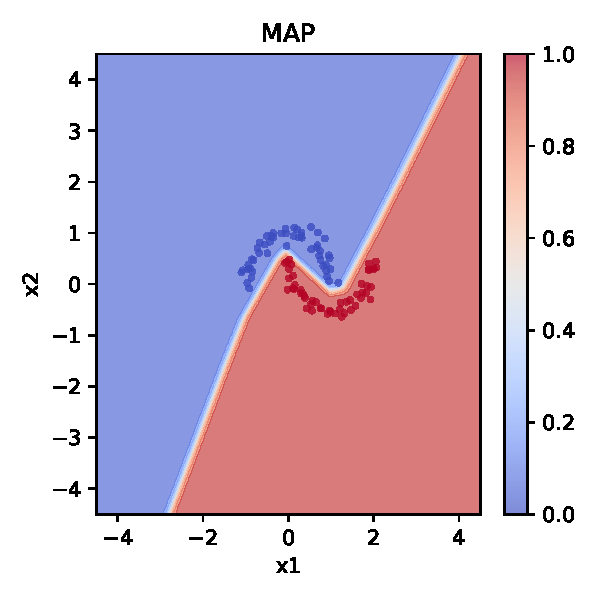
\includegraphics{images/classif_map.pdf}
  \caption{Predictions of a standard MLP. The blue and red points are training data. The color in the background represents the predicted probability $p(y \given \vec{x}, \hat{\vec{\theta}}_\text{MAP})$ at each point $\vec{x} = (x_1, x_2)^\T$ in the feature space.}
  \label{fig:classif-map}
\end{figure}

Since the network is small, we can afford computing the full Hessian matrix for Laplace approximation. In \cref{fig:classif-la}, we demonstrate the sensitivity of this method with respect to the choice of prior precision $\tau^{-2}$. For a small prior precision or large prior variance, the predictive probabilities are almost $0.5$ everywhere. The uncertainty is overestimated. As we increase the prior precision, we can recognize more meaningful structures, and the predictive distribution becomes closer to the MAP result in \cref{fig:classif-la}. A consistent pattern is that the region with predictive probabilities close to $0.5$ gets wider as we move away from the training data.

\begin{figure}[tb]
  \centering
  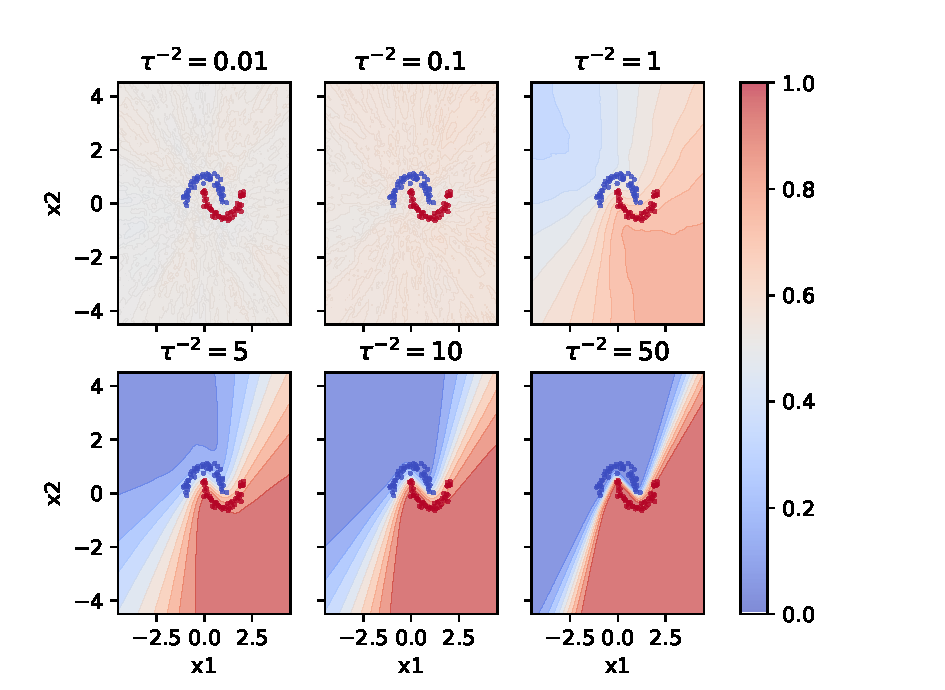
\includegraphics{images/classif_laplace.pdf}
  \caption{Laplace approximation for different prior precisions $\tau^{-2}$. Monte Carlo integration is used to approximate the predictive distribution. For each test point $(x_1, x_2)^\T$, 1000 parameters are sampled from the Gaussian approximate posterior.}
  \label{fig:classif-la}
\end{figure}

Now we construct an ensemble of 10 models with the same architecture of the MLP. The ensemble members are trained using the same hyperparameter settings, but weight initialization and batch generation are randomized. We plot five ensemble members as well as the ensemsble average in \cref{fig:classif-ensemble}. While each model is highly overconfident, some variation exists between the ensemble members. The predictive distribution given by the ensemble has a similar structure to that given by Laplace approximation with high prior precision. We observe regions of lower confidence expand towards bottom left and top right. However, the issue of overconfidence seems to persist in the other directions.

\begin{figure}[tb]
  \centering
  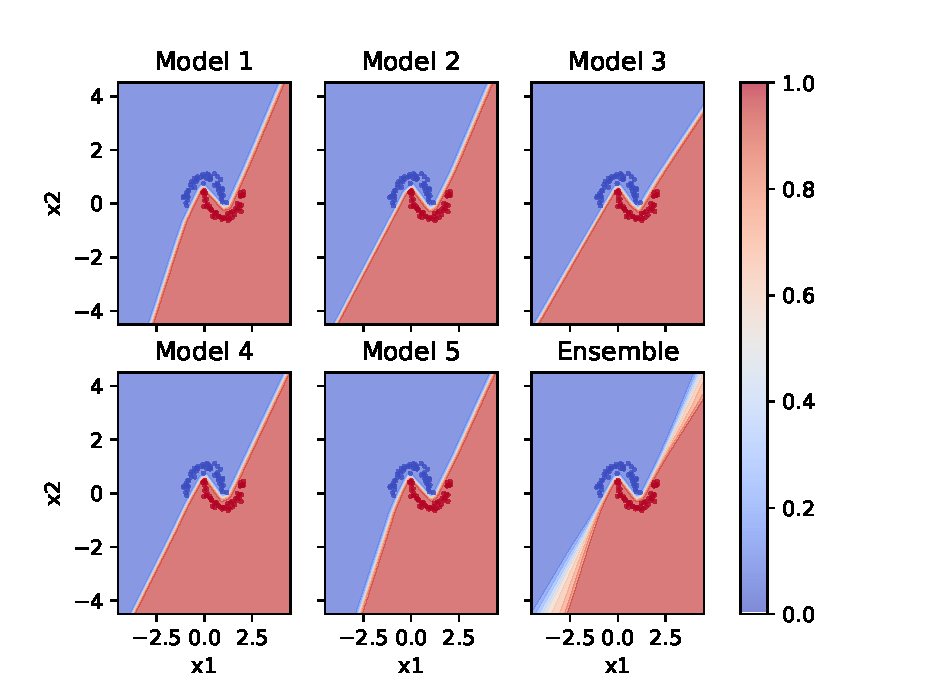
\includegraphics{images/classif_ensemble.pdf}
  \caption{Deep ensemble of 10 models. The first five plots show five individual models. The last plot shows the ensemble average.}
  \label{fig:classif-ensemble}
\end{figure}

Finally, we demonstrate Monte Carlo Dropout on the same dataset. We use the same setting to train the same MLP, but now with Dropout applied to the two hidden layers. We set the Dropout rate to $\pi = 0.2$. For such a small network, a high Dropout rate harms the prediction performance. In \cref{fig:classif-mcd}, we observe the same pattern once again: the band of low confidence extends as we move away from data, but larger regions top left and bottom right are still assigned with high confidence. We hypothesize that the unresolvable overconfidence in certain directions is a property of the network we use. \cite{kristiadiLearnableUncertaintyLaplace2021} introduced additional hidden units into the network to enhance Laplace approximation. Their approach mitigates this issue on the same dataset.

\begin{figure}[tb]
  \centering
  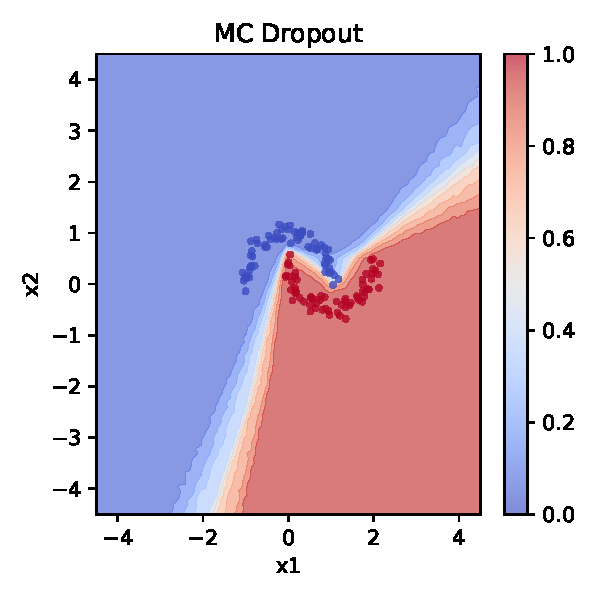
\includegraphics{images/classif_mc_dropout.pdf}
  \caption{MC Dropout. For each test point $(x_1, x_2)^\T$, a sample of 1000 parameters is used (same as for Laplace approximation).}
  \label{fig:classif-mcd}
\end{figure}

\subsection{Regression}

As a toy experiment for regression, we train an MLP with layer dimensions $[1,16,16,1]$ to learn the function $x \mapsto \sin(x)$. We generate $n = 20$ training instances as follows:
\begin{align*}
  x_i &\simiid \operatorname{Uniform}([-3, 3]), \\
  \epsilon_i &\simiid \mathcal{N}(0, 0.1^2), \\
  y_i &\defeq \sin(x) + \epsilon_i.
\end{align*}
We perform no batch generation but use standard gradient descent. The network is optimized with a learning rate of $0.1$ for 1000 epochs. The weight decay parameter is set to $10^{-6}$. \cref{fig:regr} presents the trained network (MAP estimate) and the three uncertainty quantification methods. The MAP estimate does not provide any uncertainty quantification, while we can construct error bands using the introduced methods. For Laplace Approximation, we use the last-layer variant with KFAC approximation to the Hessian and optimize the prior precision with respect to the marginal likelihood, as recommended by \cite{daxbergerLaplaceRedux2021}. The standard deviation is obtained from the Gaussian approximation to the predictive distribution. The Deep Ensemble consists of 10 models. For MC Dropout, we apply Dropout with rate $\pi = 0.2$ to both hidden layers and use the sample size 1000 for Monte Carlo integration. In the latter two approaches, we estimate the standard deviation using the empirical standard deviation over the ensemble or Monte Carlo sample.

We expect higher uncertainty when moving away from data. This is indeed observed for all three methods. Laplace Approximation is applied in a post-hoc manner. The predictive mean shown by the red curve agrees with the MAP estimate. It successfully captures the increasing uncertainty in extrapolation. Deep Ensemble exhibits higher confidence overall in comparison to Laplace approximation. \cite{lakshminarayananSimpleScalablePredictive2017b} suggests letting the model predict the error variance along with the mean, in which case overconfidence is better mitigated. The error band prodced by MC Dropout also expands when extrapolating, although not as quickly.

\begin{figure}
  \centering
  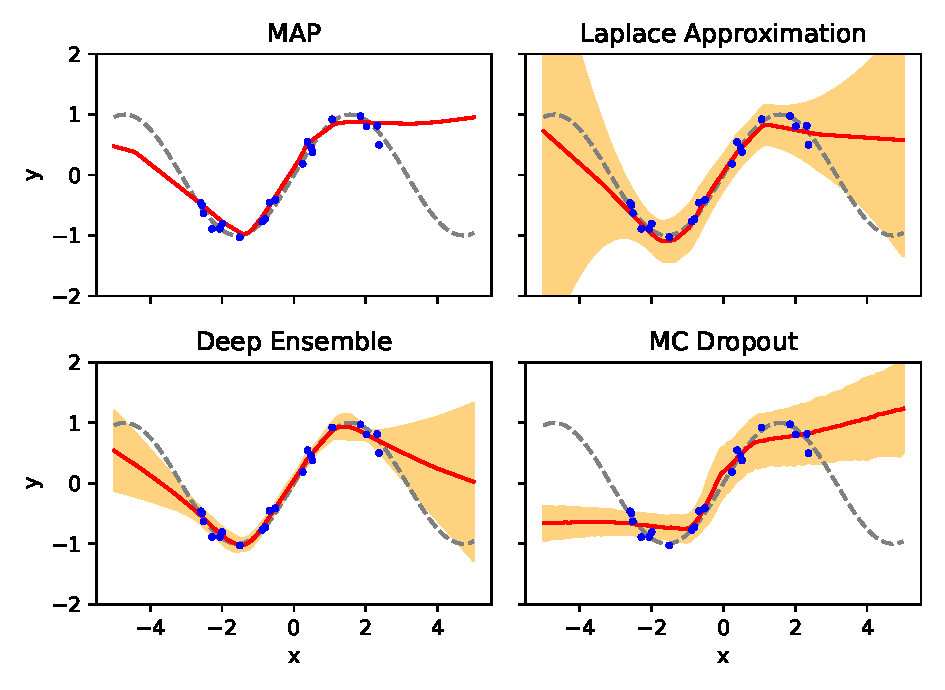
\includegraphics{images/regr_comparison.pdf}
  \caption{Comparison of MAP and uncertainty quantification methods on the regression toy dataset. The blue points as training data are sampled with Gaussian noise from the grey line. For the MAP plot, the red curve represents the prediction function. For the other plots, the predictive mean (red curve) $\pm$ two standard deviations (orange band) are shown.}
  \label{fig:regr}
\end{figure}
